\documentclass[12pt,a4paper]{article}
\usepackage[utf8]{inputenc}
\usepackage[english]{babel}
\usepackage{amsmath}
\usepackage{amsfonts}
\usepackage{amssymb}
\usepackage{graphicx}
\usepackage{tikz}
\usepackage{algorithm}
\usepackage{algorithmic}
\usepackage{listings}
\usepackage{xcolor}
\usepackage{geometry}
\usepackage{fancyhdr}
\usepackage{hyperref}

\geometry{margin=1in}
\pagestyle{fancy}
\fancyhf{}
\rhead{Dynamic Programming: Climbing Stairs}
\lhead{Algorithm Analysis}
\cfoot{\thepage}

% Code listing style
\lstset{
    language=Java,
    basicstyle=\ttfamily\small,
    keywordstyle=\color{blue},
    commentstyle=\color{green},
    stringstyle=\color{red},
    numbers=left,
    numberstyle=\tiny,
    frame=single,
    breaklines=true,
    showstringspaces=false
}

\title{\textbf{Dynamic Programming Analysis: \\The Climbing Stairs Problem}}
\author{Algorithm Implementation and Analysis}
\date{\today}

\begin{document}

\maketitle

\tableofcontents
\newpage

\section{Problem Statement}

\subsection{Definition}
The \textbf{Climbing Stairs} problem is a classic dynamic programming problem that asks: 

\begin{quote}
\textit{Given a staircase with $n$ steps, and the ability to climb either 1 or 2 steps at a time, in how many distinct ways can you reach the top?}
\end{quote}

\subsection{Mathematical Formulation}
Let $f(n)$ represent the number of ways to climb $n$ stairs. The recurrence relation is:

\begin{equation}
f(n) = \begin{cases}
1 & \text{if } n \leq 1 \\
f(n-1) + f(n-2) & \text{if } n > 1
\end{cases}
\end{equation}

This follows the Fibonacci sequence pattern, where each term is the sum of the two preceding ones.

\section{Problem Visualization}

\subsection{Small Examples}

\begin{figure}[h]
\centering
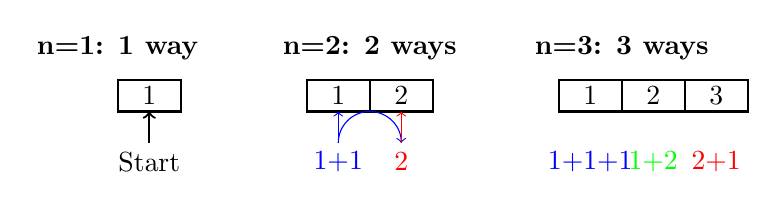
\begin{tikzpicture}[scale=0.8]
% n=1 case
\node at (0,4) {\textbf{n=1: 1 way}};
\draw[thick] (0,3) rectangle (1,3.5);
\node at (0.5,3.25) {1};
\draw[->, thick] (0.5,2.5) -- (0.5,3);
\node at (0.5,2.2) {Start};

% n=2 case
\node at (4,4) {\textbf{n=2: 2 ways}};
\draw[thick] (3,3) rectangle (4,3.5);
\draw[thick] (4,3) rectangle (5,3.5);
\node at (3.5,3.25) {1};
\node at (4.5,3.25) {2};

% Way 1: 1+1
\draw[->, blue] (3.5,2.5) -- (3.5,3);
\draw[->, blue] (3.5,2.5) arc (180:0:0.5);
\node[blue] at (3.5,2.2) {1+1};

% Way 2: 2
\draw[->, red] (4.5,2.5) -- (4.5,3);
\node[red] at (4.5,2.2) {2};

% n=3 case
\node at (8,4) {\textbf{n=3: 3 ways}};
\draw[thick] (7,3) rectangle (8,3.5);
\draw[thick] (8,3) rectangle (9,3.5);
\draw[thick] (9,3) rectangle (10,3.5);
\node at (7.5,3.25) {1};
\node at (8.5,3.25) {2};
\node at (9.5,3.25) {3};

\node[blue] at (7.5,2.2) {1+1+1};
\node[green] at (8.5,2.2) {1+2};
\node[red] at (9.5,2.2) {2+1};
\end{tikzpicture}
\caption{Visualization of climbing stairs for small values of n}
\end{figure}

\subsection{Recursive Tree Structure}

\begin{figure}[h]
\centering
\begin{tikzpicture}[level/.style={sibling distance=60mm/#1}]
\node {f(4)}
    child {
        node {f(3)}
        child {
            node {f(2)}
            child {node {f(1)}}
            child {node {f(0)}}
        }
        child {
            node {f(1)}
        }
    }
    child {
        node {f(2)}
        child {node {f(1)}}
        child {node {f(0)}}
    };
\end{tikzpicture}
\caption{Recursive call tree for f(4) showing overlapping subproblems}
\end{figure}

\section{Solution Approaches}

\subsection{Approach 1: Naive Recursion}

\begin{algorithm}
\caption{Climbing Stairs - Recursive Approach}
\begin{algorithmic}
\REQUIRE $n \geq 0$
\ENSURE Number of ways to climb $n$ stairs
\STATE \textbf{function} climbStairs($n$)
\IF{$n \leq 1$}
    \RETURN 1
\ENDIF
\RETURN climbStairs($n-1$) + climbStairs($n-2$)
\end{algorithmic}
\end{algorithm}

\textbf{Time Complexity Analysis:}
\begin{align}
T(n) &= T(n-1) + T(n-2) + O(1) \\
T(n) &= O(\phi^n) \text{ where } \phi = \frac{1+\sqrt{5}}{2} \approx 1.618
\end{align}

\textbf{Space Complexity:} $O(n)$ due to recursion stack depth.

\textbf{Problems:}
\begin{itemize}
\item Exponential time complexity
\item Redundant calculations (overlapping subproblems)
\item Stack overflow for large $n$
\end{itemize}

\subsection{Approach 2: Memoization (Top-Down DP)}

\begin{algorithm}
\caption{Climbing Stairs - Memoization}
\begin{algorithmic}
\REQUIRE $n \geq 0$, memo array initialized to 0
\ENSURE Number of ways to climb $n$ stairs
\STATE \textbf{function} climbStairsMemo($n$, memo)
\IF{$n \leq 1$}
    \RETURN 1
\ENDIF
\IF{memo[$n$] $\neq$ 0}
    \RETURN memo[$n$]
\ENDIF
\STATE memo[$n$] = climbStairsMemo($n-1$, memo) + climbStairsMemo($n-2$, memo)
\RETURN memo[$n$]
\end{algorithmic}
\end{algorithm}

\textbf{Time Complexity:} $O(n)$ - each subproblem solved exactly once \\
\textbf{Space Complexity:} $O(n)$ for memoization array + $O(n)$ recursion stack = $O(n)$

\subsection{Approach 3: Tabulation (Bottom-Up DP)}

\begin{algorithm}
\caption{Climbing Stairs - Tabulation}
\begin{algorithmic}
\REQUIRE $n \geq 0$
\ENSURE Number of ways to climb $n$ stairs
\STATE \textbf{function} climbStairsTab($n$)
\IF{$n \leq 1$}
    \RETURN 1
\ENDIF
\STATE Create array dp of size $n+1$
\STATE dp[0] = 1, dp[1] = 1
\FOR{$i = 2$ to $n$}
    \STATE dp[$i$] = dp[$i-1$] + dp[$i-2$]
\ENDFOR
\RETURN dp[$n$]
\end{algorithmic}
\end{algorithm}

\textbf{Time Complexity:} $O(n)$ \\
\textbf{Space Complexity:} $O(n)$ for DP array

\subsection{Approach 4: Space-Optimized DP}

\begin{algorithm}
\caption{Climbing Stairs - Space Optimized}
\begin{algorithmic}
\REQUIRE $n \geq 0$
\ENSURE Number of ways to climb $n$ stairs
\STATE \textbf{function} climbStairsOptimal($n$)
\IF{$n \leq 1$}
    \RETURN 1
\ENDIF
\STATE prev2 = 1, prev1 = 1
\FOR{$i = 2$ to $n$}
    \STATE current = prev1 + prev2
    \STATE prev2 = prev1
    \STATE prev1 = current
\ENDFOR
\RETURN prev1
\end{algorithmic}
\end{algorithm}

\textbf{Time Complexity:} $O(n)$ \\
\textbf{Space Complexity:} $O(1)$ - only using constant extra space

\section{Implementation Analysis}

\subsection{Java Implementation}

\begin{lstlisting}[caption=Complete Java Implementation]
public class ClimbingStairs {
    
    // Naive Recursion - O(2^n) time, O(n) space
    static int usingRecursion(int n) {
        if (n <= 1) {
            return 1;
        }
        return usingRecursion(n - 1) + usingRecursion(n - 2);
    }
    
    // Memoization - O(n) time, O(n) space
    static int dpmemoization(int n, int[] d) {
        if (n <= 1) {
            return 1;
        }
        if (d[n] != 0) {
            return d[n];
        }
        d[n] = dpmemoization(n - 1, d) + dpmemoization(n - 2, d);
        return d[n];
    }
    
    // Tabulation - O(n) time, O(n) space
    static int dpTabulation(int n) {
        if (n <= 1) return 1;
        
        int[] dp = new int[n + 1];
        dp[0] = 1;
        dp[1] = 1;
        
        for (int i = 2; i <= n; i++) {
            dp[i] = dp[i - 1] + dp[i - 2];
        }
        return dp[n];
    }
    
    // Space Optimized - O(n) time, O(1) space
    static int spaceOptimized(int n) {
        if (n <= 1) return 1;
        
        int prev2 = 1, prev1 = 1;
        for (int i = 2; i <= n; i++) {
            int current = prev1 + prev2;
            prev2 = prev1;
            prev1 = current;
        }
        return prev1;
    }
}
\end{lstlisting}

\section{Performance Comparison}

\subsection{Time Complexity Comparison}

\begin{table}[h]
\centering
\begin{tabular}{|l|c|c|c|}
\hline
\textbf{Approach} & \textbf{Time} & \textbf{Space} & \textbf{Practical Limit} \\
\hline
Naive Recursion & $O(2^n)$ & $O(n)$ & $n \leq 40$ \\
Memoization & $O(n)$ & $O(n)$ & $n \leq 10^6$ \\
Tabulation & $O(n)$ & $O(n)$ & $n \leq 10^6$ \\
Space Optimized & $O(n)$ & $O(1)$ & $n \leq 10^9$ \\
\hline
\end{tabular}
\caption{Performance comparison of different approaches}
\end{table}

\subsection{Execution Time Analysis}

For $n = 40$:
\begin{itemize}
\item \textbf{Recursion:} $\approx 1.6$ seconds
\item \textbf{Memoization:} $\approx 0.001$ seconds  
\item \textbf{Tabulation:} $\approx 0.001$ seconds
\item \textbf{Space Optimized:} $\approx 0.001$ seconds
\end{itemize}

\section{Mathematical Properties}

\subsection{Fibonacci Connection}
The climbing stairs sequence follows the Fibonacci pattern:
\begin{align}
f(0) &= 1 \\
f(1) &= 1 \\
f(2) &= 2 \\
f(3) &= 3 \\
f(4) &= 5 \\
f(5) &= 8 \\
&\vdots
\end{align}

Where $f(n) = F_{n+1}$ (the $(n+1)$-th Fibonacci number).

\subsection{Closed Form Solution}
Using Binet's formula, we can express the solution as:

\begin{equation}
f(n) = \frac{\phi^{n+1} - \psi^{n+1}}{\sqrt{5}}
\end{equation}

Where:
\begin{align}
\phi &= \frac{1 + \sqrt{5}}{2} \approx 1.618 \text{ (Golden Ratio)} \\
\psi &= \frac{1 - \sqrt{5}}{2} \approx -0.618
\end{align}

\section{Extensions and Variations}

\subsection{Generalized Problem}
\textbf{Problem:} Climb stairs with steps of size 1, 2, or 3.

\textbf{Recurrence:}
\begin{equation}
f(n) = \begin{cases}
1 & \text{if } n = 0 \\
1 & \text{if } n = 1 \\
2 & \text{if } n = 2 \\
f(n-1) + f(n-2) + f(n-3) & \text{if } n > 2
\end{cases}
\end{equation}

\subsection{Cost Minimization}
\textbf{Problem:} Each step has a cost, find minimum cost to reach top.

\textbf{Recurrence:}
\begin{equation}
cost(n) = \min(cost(n-1) + c_1, cost(n-2) + c_2)
\end{equation}

\section{Conclusion}

The Climbing Stairs problem demonstrates the power of dynamic programming in optimizing recursive solutions:

\begin{enumerate}
\item \textbf{Pattern Recognition:} Identifying the Fibonacci-like recurrence relation
\item \textbf{Optimization Strategy:} Eliminating redundant calculations through memoization
\item \textbf{Space Optimization:} Reducing space complexity from $O(n)$ to $O(1)$
\item \textbf{Practical Applications:} Understanding trade-offs between time and space
\end{enumerate}

\textbf{Key Takeaways:}
\begin{itemize}
\item Always analyze the problem for overlapping subproblems
\item Consider both top-down (memoization) and bottom-up (tabulation) approaches
\item Look for opportunities to optimize space complexity
\item Understand the mathematical foundations behind the algorithm
\end{itemize}

\section{References}

\begin{enumerate}
\item Cormen, T. H., Leiserson, C. E., Rivest, R. L., \& Stein, C. (2009). \textit{Introduction to Algorithms} (3rd ed.). MIT Press.
\item Kleinberg, J., \& Tardos, E. (2005). \textit{Algorithm Design}. Addison-Wesley.
\item Dynamic Programming Problems on LeetCode: Problem 70 - Climbing Stairs
\end{enumerate}

\end{document}
